In Section~\ref{sec:equipment_bonuses} we discussed the basic formulation of equipment bonuses. In this chapter, we will be interested in optimizing the player's choice of equipment to maximize some metric. Some examples of these metrics would be combat experience per hour, number of kills per hour, probability of winning, and so. Since the goal of the player may vary heavily, we aim to produce a general framework that can maximize arbitrary objective functions.

There are a large number of items that a player can equip in each slot, typically ranging from 10-100 considerations. Exhaustively considering each possible combination of equipment would result in roughly $10^{10}$ to $100^{10}$ possible sets. It is obvious then, that brute force would not work. We aim to reduce the number of possible equipments \textit{loadouts}, $\mathcal{L}$ that we must consider. A loadout is simply the set of equipment that a fighter is wearing:
\begin{align}
	\mathcal{L} = \{I_\text{slot}\,|\,\text{slot} \in \text{slots}\}.
\end{align}
To do this, we will reduce redundant equipment choices for each slot such that we end with a set of \emph{possibly} optimal loadouts. The only way to determine which of those is the actual optimal solution, $\mathcal{L}^*$ is to numerically evaluate the value of the objective, $f$, for each possibly optimal loadout. This defines our optimization problem as:
\begin{align}
	\mathcal{L}^* \leftarrow \mathop{\mathrm{argmin}}_{\mathcal{L} \in \{\mathcal{L}\}} f(\mathcal{L}).
\end{align}
So we will begin by reducing the size of the set $\{\mathcal{L}\}$.

\section{The Projection Vector}
	Different optimization problems require different information about the player's equipment. For example, when straightforwardly optimizing pure damage output (typically measured in kills per hour), the defensive bonuses of the player are irrelevant. By contrast, trying to maximize the probability of killing an opponent would require consideration of those defensive bonuses. Furthermore, a fighter only attacks with one attack style at a time. So clearly, not all bonuses are required for every optimization. For this reason, we introduce a \textit{projection} vector, $\vec{p}$, that will \emph{select} the bonuses that matter. Recall that our bonuses are divided into two groups: constant bonuses, and special bonuses. In Section~\ref{sec:equipment_bonuses}, we discussed how we treat special bonuses differently. So we will ignore them for now, and focus on the constant bonuses, $\vec{\mathcal{I}}_c^\text{slot}$. To select out the desired bonuses, we make $\vec{p}$ the same length as $\vec{\mathcal{I}}_c^\text{slot}$ so that each element in $\vec{p}$ corresponds to an equipment bonus. We can do so-called one-hot encoding, where we set elements to either 0 or 1 depending on whether the corresponding equipment bonus should be considered.

	An element-wise multiplication (also known as a Hadamard product) of these two vectors, $\vec{\mathcal{I}}_c^\text{slot} \odot \vec{p}$ contains the bonuses of the item that we want, and 0's for bonuses we don't want to consider. To compare different items we need to define a comparison operator, $\hat C (\cdot, \cdot)$ such that:
	\begin{align}
	    \hat C (\vec{\mathcal{I}}_{c, 1}^\text{slot}, \vec{\mathcal{I}}_{c, 2}^\text{slot}; \vec{p}) = \begin{cases}
	        1 \text{ if $\exists\,i\in [1, n]\,|\,(\vec{\mathcal{I}}_{c, 1}^\text{slot}  \odot \vec p)_i > (\vec{\mathcal{I}}_{c, 2}^\text{slot}  \odot \vec p)_i$} \\
	        0 \text{ otherwise},
	    \end{cases}
	\end{align}
	where $n$ is the number of bonuses for an item can have, and $(\cdot)_i$ represents the $i$'th bonus.
	By simply comparing the individual item bonuses, this term indicates whether some item, $\vec{\mathcal{I}}_{c, 1}^\text{slot}$, provides some advantage over another, $\vec{\mathcal{I}}_{c, 2}^\text{slot}$. If a given item doesn't provide some advantage over any other item then it doesn't need to be included in the set of equipment to consider. Note that $\hat C (\vec{\mathcal{I}}_{c, 1}^\text{slot}, \vec{\mathcal{I}}_{c, 1}^\text{slot}; \vec{p}) = 0$.

\section{Set Reduction}
	With this, we can reduce the set of possible items in given slot, $\{\mathcal{I}^\text{slot}_j\}_{j=1}^{N_\text{slot}}$, where $N_\text{slot}$ is the number of possible items in that slot. We can define the following matrix,
	\begin{align}
	    \boldsymbol{A}^{\vec{p}} = A_{ij}^{\vec{p}} = \hat C (\vec{\mathcal{I}}_{c, i}^\text{slot}, \vec{\mathcal{I}}_{c, j}^\text{slot}; \vec{p}),
	\end{align}
	that is also one-hot encoded with 1's representing that the item in column $i$ provides some advantage over the item in row $j$, for our optimization problem.

	These individual item comparisons aren't too important, instead we care if an item may provide some advantage over \emph{any} other in the set. So, an item shouldn't be considered if the comparison yields 0 when compared against all other items:
	\begin{align}
	    &\sum_{i=1}^N \hat C (\vec{\mathcal{I}}_{c, j}^\text{slot}, \vec{\mathcal{I}}_{c, i}^\text{slot}; \vec{p}) = 0\\
	    \implies&\sum_{i=1}^N A_{ij}^{\vec{p}} = 0\\
	    \implies&\boldsymbol{1}\cdot\boldsymbol{A}_j^{\vec{p}} = 0
	\end{align}
	where $\boldsymbol{1}$ is a $N_\text{slot}$-dimensional vector containing ones, and $\boldsymbol{A}_j^{\vec{p}}$ is the $j$'th column in $\boldsymbol{A}^{\vec{p}}$.
	Then the reduced set of items for a given slot is then:
	\begin{align}
	    \{\mathcal{I}^\text{slot}_j; \vec{p}\}_{j=1}^{\bar{N}_\text{slot}} = \{\mathcal{I}_j^\text{slot}\,|\,\boldsymbol{1}\cdot\boldsymbol{A}_j^{\vec{p}} \neq 0,\,\,\, 1 \leq j \leq N_\text{slot}\},
	\end{align}
	where $\bar{N}_\text{slot}$ is the number of items left in this reduced set. The possibly optimal loadout set can be constructed as a ``$n$-ary'' Cartesian product:
	\begin{align}
		\{\bar{\mathcal{L}}; \vec{p}\} = \{(\mathcal{I}^\text{head}, ..., \mathcal{I}^\text{ring}) | \mathcal{I}^\text{slot} \in \{\mathcal{I}^\text{slot}_j; \vec{p}\}_{j=1}^{\bar{N}_\text{slot}} \,\forall\, \text{slot} \in \{\text{slots}\}\}
		% \{\mathcal{I}^\text{slot}_j; \vec{p}\}_{j=1}^{\bar{N}_\text{slot}}
	\end{align}
	% In future, it would be nice to see an example matrix for some arbitrary slot.

	As mentioned earlier, the choice of $\vec p$ depends on the problem at hand. However, only one attack style is generally considered and so often $\vec p$ can be chosen to only consider one attack style.\footnote{If the fighter switches weapons, or has multiple attacks, considering more than one attack style would then be required.} A natural formulation would be to iterate over each attack style. We can, for example, use $\vec{p}_\text{stab}$ to denote a projection vector which has stab as the only non-zero attack bonus. Then, the total set of considerations is the union of the specific attack style sets:
	% and disregarding weapons that cannot be used.
	\begin{align}
	    \{\bar{\mathcal{L}}; \vec{p}\} = \bigcup_{a\in \{\text{attack styles}\}}  \{\bar{\mathcal{L}}; \vec{p_a}\}.
	\end{align}
	This makes our optimization:
	\begin{align}
		\mathcal{L}^* \leftarrow \mathop{\mathrm{argmin}}_{\mathcal{L} \in \{\bar{\mathcal{L}}; \vec{p}\}} f(L),
	\end{align}
	which has reduced a search space containing billions of possibilities to one containing (empirically) less than 1,000.


	% (unless the fighter switches attack styles during the fight), only one



\section{Gear Optimization Implementation \& GUI}
	The ability to determine the optimal gear load-out for a given player-opponent-environment combination is possible through the previous sections. Set reduction makes brute force feasible albeit with special equipment complicating the implementation. With a reduced set, one can simply evaluate the theoretical calculations for the desired metric (eg: xp/h, kills per hour, $P_\text{win}$) for every ``possibly-optimal'' gear load-out. The solution is simply the load-out with the maximum value. The full interface with all considerations is shown in Fig.~\ref{fig:gear_optimizer}.

	\begin{figure}
		\centering
		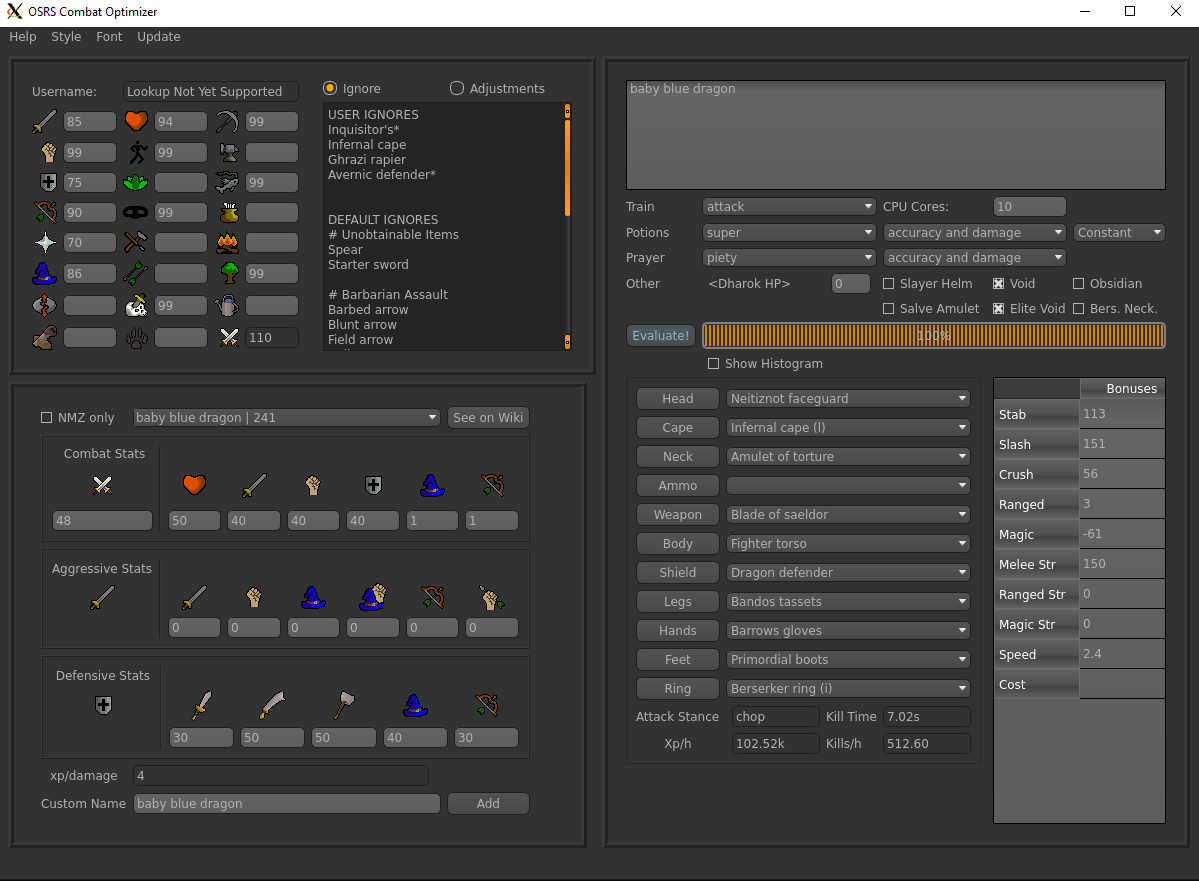
\includegraphics[width=\linewidth]{img/combat/gear_optimizer.png}
		\caption{
			The optimal equipment gear optimizer tool written in PyQt5. The user inputs their skill levels, which not only determine combat skills but also auxiliary skill requirements (eg: combat axes require woodcutting levels). The player can iteratively ignore items as the optimal solution suggests items the player cannot obtain. The panel for level requirements and stat adjustments is hidden. On the bottom, the player also selects their opponent and respective stats; they can also add multiple opponents to be fought in sequence. Environmental information (eg: potions, slayer task), along with which skill to train can be selected in the top right. CPU cores reflects the multi-threaded implementation which brute forces over the reduced equipment sets. Finally, the optimal item is identifier for each equipment slot, which is stated alongside the bonuses and metrics. Special equipment effects are only partially treated, which can impact the reliability, however it should be considered accurate for all normal combat.
		}
		\label{fig:gear_optimizer}
	\end{figure}

